\documentclass{technical_presentation}

\title{Technical Presentation Template}
\subtitle{Wow much subtitle}

\author{Kai Takac}
\date{ENI, 2019}

\begin{document}

%% Title %%%%%%%%%%%%%%%%%%%

\begin{frame}
	\titlepage
\end{frame}

%% Content %%%%%%%%%%%%%%%%%%%


\section{Some Basics}

% Telling a story

\begin{frame}[shrink]
	\frametitle{A lot of text with smaller font size}
	Lorem ipsum dolor sit amet, consetetur sadipscing elitr, sed diam nonumy eirmod tempor invidunt ut labore et dolore magna aliquyam erat, sed diam voluptua. At vero eos et accusam et justo duo dolores et ea rebum. Stet clita kasd gubergren, no sea takimata sanctus est Lorem ipsum dolor sit amet. Lorem ipsum dolor sit amet, consetetur sadipscing elitr, sed diam nonumy eirmod tempor invidunt ut labore et dolore magna aliquyam erat, sed diam voluptua. At vero eos et accusam et justo duo dolores et ea rebum. Stet clita kasd gubergren, no sea takimata sanctus est Lorem ipsum dolor sit amet.
\end{frame}

\begin{frame}
	\frametitle{Some Basics}
	
	\begin{itemize}
		\item Put stuff in frames
		\begin{itemize}
			\item Sub-point
		\end{itemize}
	\end{itemize}
\end{frame}

\section{Some Example Slides}

% German
\begin{frame} 
    \frametitle{Umlaute Test}
    %Content goes here
    Hallo wie geht es dir.
    Test mit Sonderzeichen ÖÄÜ.
    
    \footnote{Fußnoten: test foot note}
\end{frame}

% References
\begin{frame}
    \frametitle{References Test}
    \framesubtitle{A bit more information about this}
    
    References and literature are provided through babel.
    There are different quotation and referencing styles \cite{hgb2019latex}.
    %More content goes here
\end{frame}
  
\begin{frame}[fragile]
	\frametitle{Source Code}
  	
  	 As you can see in the following block, code highlighting is also working!
  	 
  	 \begin{minted}{c} 
int main() {
	printf("hello, world");
	return 0;
}
	\end{minted}
  	
\end{frame}

\subsection{Math}

\begin{frame}
	\frametitle{Math}

	\begin{itemize}
		\item This is a math expression $x=10.5$
	\end{itemize}

\end{frame}

% Figures

\subsection{Figures}

\begin{frame}
	\frametitle{This frame has a top and bottom bar}
	\centering
	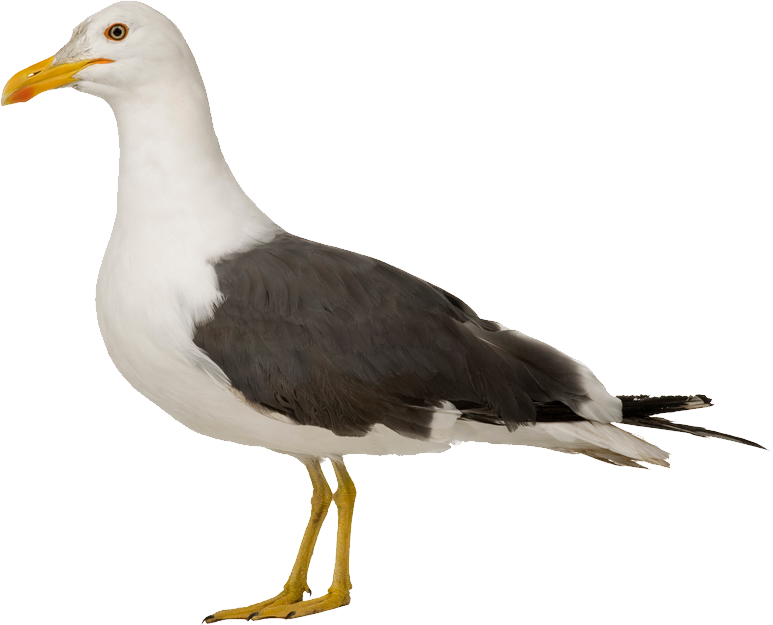
\includegraphics[height=0.8\textheight]{figures/gull}
\end{frame}

\begin{frame}[plain]
	\centering
	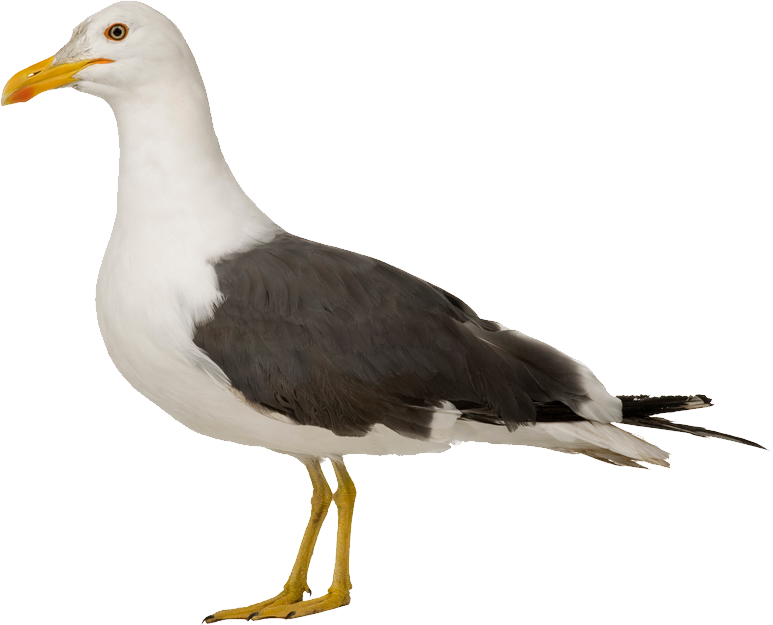
\includegraphics[height=\textheight]{figures/gull}
\end{frame}
  

% etc

% References %%%%%%%%%%%%%%%%%%%%%%%

\appendix

\begin{frame}[allowframebreaks]
	\frametitle{References}
	\printbibliography[heading=bibintoc]
\end{frame}

\end{document}